\documentclass[11pt,a4paper]{article}
\usepackage[margin=2.2cm]{geometry}
\usepackage{times}
\usepackage{booktabs}
\usepackage{tabularx}
\usepackage{array}
\usepackage{graphicx}
\usepackage{hyperref}
\usepackage{setspace}
\usepackage{enumitem}
\usepackage{caption}
\usepackage[T1]{fontenc}
\usepackage{float} 

\hypersetup{colorlinks=true, linkcolor=black, urlcolor=blue, citecolor=black}
\setstretch{1.12}
\setlength{\parskip}{0.4em}
\setlength{\parindent}{0pt}
\captionsetup{font=small}

\title{\textbf{Task 1:} Research Proposal, Related Work Matrix, Litmap \\and Literature Synthesis}
\author{Irgimbayev Adi \and Shmyrin Alan}
\date{\today}

\begin{document}
\maketitle

\section{Methodology Card}

\textbf{Research topic.}
The Effect of Generative AI-Assisted Programming on Critical Thinking and Academic Performance of Undergraduate IT Students.

\textbf{Object of research.}
The learning process of undergraduate students in IT and computer science programs, especially in programming courses.

\textbf{Subject of research.}
How generative AI-assisted programming (by intensity and by manner of use) is related to students' critical thinking and academic performance.

\textbf{Research aim.}
To examine how the use of generative AI in programming education is linked to critical thinking and academic performance among undergraduate IT students, with attention to both how often students use AI and how they use it.


\subsection*{Research questions}
\begin{enumerate}[leftmargin=*, itemsep=0.2em]
  \item[\textbf{RQ1}] How does the use of generative AI during programming tasks affect the critical thinking performance of undergraduate IT students?
  \item[\textbf{RQ2}] What is the relationship between the intensity of generative AI use and the academic performance of undergraduate IT students?
  \item[\textbf{RQ3}] Does the way students use generative AI affect their critical thinking and academic performance?
\end{enumerate}

\subsection*{Hypotheses and Testable Variables}

\paragraph{RQ1 Hypotheses and Variables.}
\begin{itemize}[leftmargin=*, itemsep=0.1em]
  \item \textbf{H0:} Generative AI use during programming tasks does not significantly affect students' critical thinking performance.
  \item \textbf{H1:} Generative AI use during programming tasks significantly affects students' critical thinking performance.
  \item \textbf{Independent Variable (IV):} Generative AI use during coding tasks (binary/categorical usage mode).
  \item \textbf{Dependent Variable (DV):} Critical thinking performance score (measured via validated critical thinking assessments/rubrics).
  \item \textbf{Controlled Variables (CV):} Prior programming knowledge, year of study, cumulative GPA, prior coding experience, time spent on task, task difficulty level.
\end{itemize}

\paragraph{RQ2 Hypotheses and Variables.}
\begin{itemize}[leftmargin=*, itemsep=0.1em]
  \item \textbf{H0:} There is no statistically significant relationship between the intensity of generative AI use and academic performance.
  \item \textbf{H1:} There is a statistically significant relationship between the intensity of generative AI use and academic performance.
  \item \textbf{Independent Variable (IV):} Intensity of generative AI use (frequency of interaction, proportion of AI-assisted code steps).
  \item \textbf{Dependent Variable (DV):} Academic performance (assignment grades, practical test scores, course final grade).
  \item \textbf{Controlled Variables (CV):} Baseline GPA, prior programming experience, year of study, initial subject knowledge, task difficulty, individual study time.
\end{itemize}

\paragraph{RQ3 Hypotheses and Variables.}
\begin{itemize}[leftmargin=*, itemsep=0.1em]
  \item \textbf{H0:} The manner of generative AI use does not significantly affect critical thinking or academic performance.
  \item \textbf{H1:} Students who primarily use generative AI for explanations and debugging feedback demonstrate higher critical thinking and academic performance scores than those who primarily use AI for full solution generation.
  \item \textbf{Independent Variable (IV):} Manner/type of AI use (explanation/conceptual feedback mode vs. direct solution/code generation mode).
  \item \textbf{Dependent Variables (DV):} Critical thinking assessment score, programming assignment score, overall academic performance.
  \item \textbf{Controlled Variables (CV):} Prior programming proficiency, baseline GPA, coding experience, year of study, task completion time, assignment complexity.
\end{itemize}

\subsection*{FINER Criteria Assessment}
The proposed research questions satisfy the FINER framework criteria:
\begin{itemize}[leftmargin=*, itemsep=0.2em]
  \item \textbf{Feasible:} We can carry out this research within a standard academic semester by surveying undergraduate IT students, analyzing their coursework performance, and using established critical thinking tests.
  \item \textbf{Interesting:} It addresses a key concern for students and professors today: whether AI tools actually help students learn programming or just lead to lazy thinking and cognitive offloading.
  \item \textbf{Novel:} Most existing papers look at coding grades or critical thinking separately. Our study combines both and specifically separates the intensity of AI use from the type of use (e.g., asking for explanations vs. copying ready code).
  \item \textbf{Ethical:} Participation will be completely voluntary, student responses and data will be anonymized, and all steps will follow university academic integrity policies.
  \item \textbf{Relevant:} The results will help educators create practical rules for using GenAI in programming classes without losing core problem-solving skills.
\end{itemize}

\subsection*{Research tasks}
\begin{enumerate}[leftmargin=*, itemsep=0.15em]
  \item Review research on generative AI in programming education, critical thinking, and academic performance.
  \item Design a methodology for measuring AI-use intensity, AI-use type, critical thinking, and academic performance.
  \item Collect data on students' AI usage patterns and learning outcomes.
  \item Analyze the empirical relationships stated in RQ1--RQ3 while controlling for background variables.
  \item Draw conclusions and propose practical recommendations for GenAI integration in IT programming courses.
\end{enumerate}

\section{Related Work Comparison Matrix}

\begin{table}[H]
\centering
\small
\renewcommand{\arraystretch}{1.1}
\caption{Comparison of key related works selected from our ResearchRabbit collection (52 unique sources).}
\label{tab:matrix}
\begin{tabularx}{\textwidth}{@{}>{\raggedright\arraybackslash}p{2.35cm}>{\raggedright\arraybackslash}p{2.45cm}>{\raggedright\arraybackslash}p{2.35cm}>{\raggedright\arraybackslash}p{2.15cm}>{\raggedright\arraybackslash}X@{}}
\toprule
\textbf{Source} & \textbf{Method / focus} & \textbf{Context} & \textbf{Main metrics} & \textbf{Limitation for our study} \\
\midrule
Zhou et al.\ (2024) & Quantitative mediation study & Higher education; GenAI self-regulation & Critical thinking; problem-solving & Not focused on IT programming tasks or AI-use modes in coding \\
\addlinespace
Suriano et al.\ (2024) & Empirical study of ChatGPT interaction & Student learning settings & Complex critical thinking skills & Limited link to programming course grades and AI intensity \\
\addlinespace
Larson et al.\ (2024) & Conceptual analysis & GenAI and critical thinking & Framing of risks and opportunities & Not an empirical IT-programming experiment \\
\addlinespace
Kassenkhan et al.\ (2025) & Review of AI and gamification & Education systems & Strategies for critical thinking & Broad education focus; weak programming-performance evidence \\
\addlinespace
Baig et al.\ (2026) & Literature review & ChatGPT in programming education & Applications and reported outcomes & Review format; does not test intensity vs manner of use \\
\addlinespace
Gambo et al.\ (2026) & Mixed-methods study & University programming courses & Learning outcomes; performance & Does not clearly separate explanation use from solution generation \\
\addlinespace
Denny et al.\ (2024) & Intervention on prompting and comprehension & Computing education & Code comprehension; prompting skills & Critical thinking and AI intensity are not jointly modeled \\
\addlinespace
Nasr et al.\ (2025) & Exploration of GenAI and critical thinking & Higher education & Critical thinking outcomes & Not specific to undergraduate IT programming coursework \\
\bottomrule
\end{tabularx}
\end{table}

\section{Literature Review Synthesis}

Generative AI tools are already common in undergraduate study, including programming courses. Reviews and course studies show that ChatGPT can support coding tasks and change how students ask for help, complete assignments, and report learning gains~\cite{chatgpt_baig_2026,impact_gambo_2026,explaining_denny_2024}. At the same time, a large part of the recent literature is concerned with critical thinking: whether AI helps students reason better, or whether it encourages shallow answers and cognitive offloading~\cite{critical_larson_2024,ai_gerlich_2025,artificial_zer_2025}.

Three themes are especially useful for our topic. First, programming-education work suggests that GenAI can improve short-term performance and code-related support, but the quality of learning depends on how students prompt and check AI output~\cite{chatgpt_baig_2026,impact_gambo_2026,explaining_denny_2024}. Second, critical-thinking studies show that interaction with ChatGPT may promote complex reasoning when students actively evaluate responses, and that self-regulation can mediate the link between GenAI use and thinking outcomes~\cite{student_suriano_2024,mediating_zhou_2024,prompts_yang_2025}. Third, broader education reviews connect AI tools, gamification, and classroom design to critical thinking, but often outside IT-specific programming assessment~\cite{gamification_kassenkhan_2025,exploring_nasr_2025,collaborative_ruizrojas_2024}.

The research gap is still clear. Many papers discuss either programming performance or critical thinking, but few designs for undergraduate IT students measure both together while separating intensity of AI use from manner of use. In other words, we still lack strong evidence on whether explanation-oriented AI use supports critical thinking better than full-solution generation, and whether heavier AI use is associated with higher academic performance after controlling for prior knowledge and study time.

This study addresses that gap in alignment with the FINER criteria. We focus on undergraduate IT students and examine generative AI-assisted programming through intensity and type of use, then link these patterns to critical thinking and academic performance (RQ1--RQ3). The aim is to connect computing-education findings with critical-thinking research and to support practical recommendations for GenAI use in programming courses.

\vspace{0.3em}

\section{Literature Network Map and Shared Links}

\subsection*{ResearchRabbit LitMap}
Public share link:\\
\url{https://app.researchrabbit.ai/folder-shares/9e966e1f-0b0c-438c-87c5-dd65195366e1}

\noindent Our ResearchRabbit collection comprises 20 curated bibliographic records selected for final mapping and analysis. Landmark papers anchoring this network include Zhou et al.\ (2024), Suriano et al.\ (2024), Larson et al.\ (2024), Baig et al.\ (2026), and Gambo et al.\ (2026).

\subsection*{LitMap screenshot}
\begin{figure}[H]
\centering
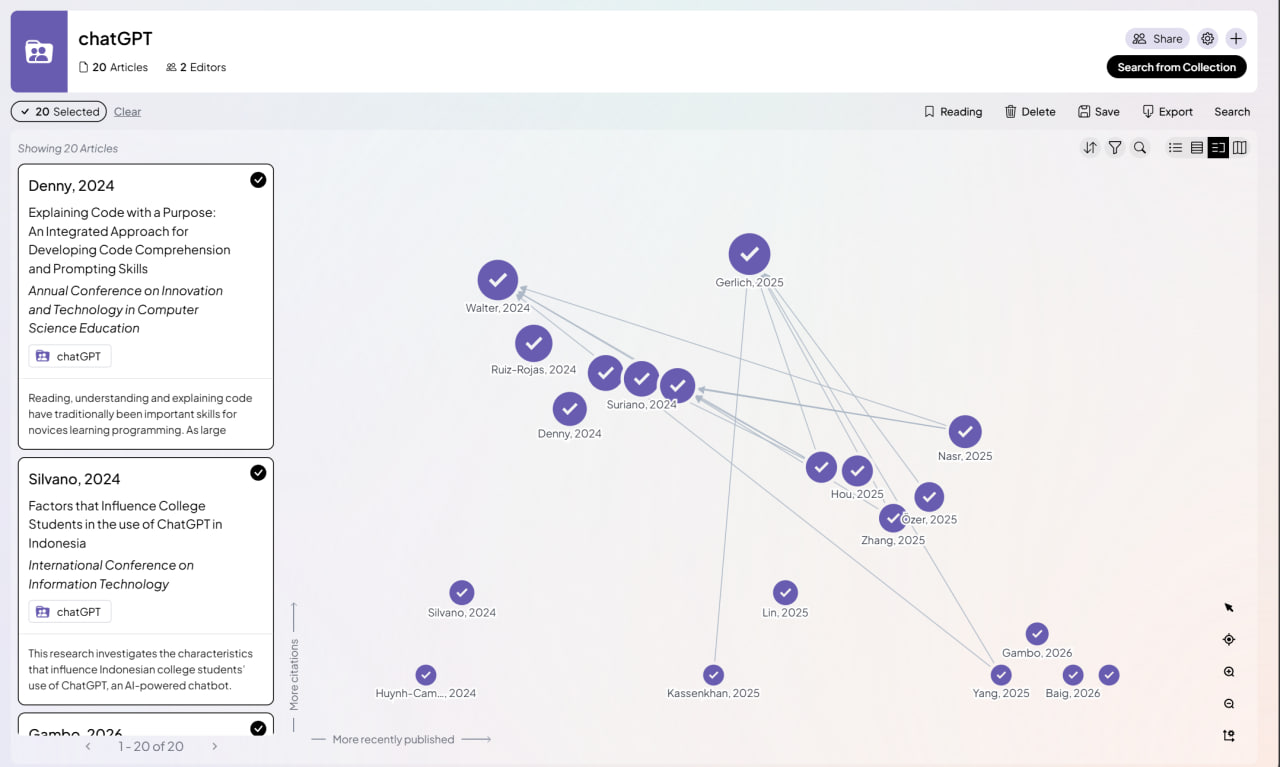
\includegraphics[width=0.92\textwidth]{litmap1.png}
\caption{Literature network map from the shared ResearchRabbit collection.}
\label{fig:litmap}
\end{figure}

\subsection*{Zotero library}
\begin{itemize}[leftmargin=*]
  \item Collection name: \texttt{Methods\_Adi\_Alan}
  \item Shared collection link: \url{https://www.zotero.org/groups/6692752/methods_adi_alan/library}
  \item BibTeX file: \texttt{references.bib}
\end{itemize}

\subsection*{GitHub source}
Repository URL: \url{https://github.com/Irgimbayev/Methods_Adi_Alan}

\bibliographystyle{ieeetr}
\bibliography{references}

\end{document}